\documentclass[11pt,letterpaper]{article}

\usepackage{textcomp}
\usepackage{fullpage}
\usepackage{amsfonts}
\usepackage{verbatim}
\usepackage[english]{babel}
\usepackage{pifont}
\usepackage{color}
\usepackage{setspace}
\usepackage{lscape}
\usepackage{indentfirst}
\usepackage[normalem]{ulem}
\usepackage{booktabs}
%\usepackage{nag}
\usepackage{natbib}
%\usepackage{bibtex}
\usepackage{float}
\usepackage{latexsym}
%\usepackage{hyperref} 
\usepackage{url}
%\usepackage{html}
\usepackage{hyperref}
\usepackage{epsfig}
\usepackage{graphicx}
\usepackage{amssymb}
\usepackage{amsmath}
\usepackage{bm}
\usepackage{array}
\usepackage{mhchem}
\usepackage{ifthen}
\usepackage{caption}
\usepackage{hyperref}
%\usepackage{xcolor}
\usepackage{amsthm}
\usepackage{amstext}
\usepackage{lineno}

\usepackage{sectsty,setspace,natbib}
\usepackage[top=1.00in, bottom=1.0in, left=1in, right=1.25in]{geometry}
\usepackage{graphicx}
\usepackage{latexsym,amssymb,epsf,rotating}
\usepackage{epstopdf}
\usepackage{amsmath}
\usepackage{natbib}
\usepackage{todonotes}
\usepackage{framed}

\linespread{1.2} % was 1.66 for double-spaced 
% \raggedright
\setlength{\parindent}{0.5in}

\setcounter{secnumdepth}{0}
% Our sections are not numbered and our papers do not have
% Tables of Contents. We don't 
% present a list of figures or list of tables, either.

% Any common font is fine.
% (A common sans-serif font should be used on figures, but figures should be
% separate from the LaTeX document.)

\pagestyle{empty}

\renewcommand{\section}[1]{%
\bigskip
\begin{center}
\begin{Large}
\normalfont\scshape #1
\medskip
\end{Large}
\end{center}}

\renewcommand{\subsection}[1]{%
\bigskip
\begin{center}
\begin{large}
\normalfont\itshape #1
\end{large}
\end{center}}

\renewcommand{\subsubsection}[1]{%
\vspace{2ex}
\noindent
\textit{#1.}---}

\renewcommand{\tableofcontents}{}

\bibpunct{(}{)}{;}{a}{}{,}  % this is a citation format command for natbib

\parskip=5pt
\pagenumbering{arabic}
\pagestyle{plain}

\begin{document}
\begin{flushright}
Version dated: \today
\end{flushright}
\bigskip
\noindent RH: Interactive cues and spring phenology
% put in your own RH (running head)

\bigskip
\medskip
\begin{center}

% Insert your title:
\noindent{\Large {\bf Concept paper on understanding interactive cues and climate change (with growth chamber studies)}}\\
\vspace{2ex}
{\Large (1) How interactive cues will shape climate change responses \\
\vspace{2ex}
(2) Limiting cues: How spring warming, winter chilling and daylength will shape climate change responses\\
\vspace{2ex}
(3) Spring warming, winter warming or daylength: What cue will be most limiting in future tree phenology?} % What cue will be most limiting with climate change? Forcing x photoperiod x chilling
% Isabelle likes 3 best.
\bigskip

\noindent {\normalsize \sc
The lab$^{1,2}$}\\
\noindent {\small \it
$^1$ Arnold Arboretum of Harvard University, 1300 Centre Street, Boston, Massachusetts, 02131, USA\\
$^2$ Organismic \& Evolutionary Biology, Harvard University, 26 Oxford Street, Cambridge, Massachusetts, 02138, USA\\
$^3$ Forest \& Conservation Sciences, Faculty of Forestry, University of British Columbia, 2424 Main Mall, Vancouver, BC V6T 1Z4}\\

\end{center}
\medskip
\noindent{\bf Corresponding author:} XX, see $^{1,2}$ above ; E-mail:.\\

\newpage
%\linenumbers

\begin{abstract}
Climate change has shifted plant phenology globally, with average shifts of 4-6 days/\textdegree C and some species shifting several weeks. Globally, such shifts have been some of the most reported and most predictable biological impacts of climate change. This predictability comes from decades of research, which have outlined the major cues that drive most studied plant phenology: temperatures (including spring warming and winter chilling) and daylength. Further simplifying predictions, spring temperatures are often the dominant cue in nature, making linear models of heat sums often excellent at predicting interannual variation in phenology. Yet as climate change has marched on, new research has uncovered failures to predict the current observed changes, with many shifts appearing more muted over certain time periods or in certain locations. Here we argue that such inaccurate predictions are most likely due to simple models that neglect to consider other major cues---especially winter chilling and daylength, which moderate and shape plant phenological responses to spring warming. We highlight how over 60 years of research in controlled environments can improve predictions for when, where and how the interactive effects of other cues will impact simple linear predictions. Finally, we discuss how a new generation of controlled environment experiments could rapidly improve our predictive capacity for woody plant phenology in coming decades.  
\end{abstract}

\noindent \emph{Main message (and, really, it's important):} If you want to project climate change impacts, you need to focus on relevant changes in all three cues. The relevant changes part is about comparing cues, the all three cues is about interactive cues.

\noindent \emph{Keywords:} phenology, climate change, spring warming, forcing, chilling, daylength, photoperiod, non-linear responses, leafout, budburst\\

\newpage
\noindent {\bf Some to do items}
\begin{enumerate}
\item Need to double-check how I count cues for checking INTERACTIONS!
\item Parse out the multiple types of non-linearities better and see if we can show an example of a double-cue non-linearity (Flynn data?)
\item Add details on exactly how figure 1 was created.
\item See question in 4d.
\item What figures do we really need/want in paper?
\item Check 5d ... do 43\% of the studies really vary photo and force?
% \item Totally random idea: Should we do a really small subset of species and try to do interactions?
\end{enumerate}


\noindent {\bf Take home messages}
\begin{enumerate}
\item Current studies are relevant for some single cues ...
\item Interactive cues
\item Long-term studies should work harder to integrate experimental results... 
\end{enumerate}



\section{Outline}
% Ask yourself: What do people need to do to fit better models and predict limits to shifts?
% \citep{delpierre2009}: Not sure where to cite this. 
\begin{enumerate}
\item Introduction 
\begin{enumerate}
\item Shifts in spring phenology are one of the most reported and most predictable changes with climate change
\begin{enumerate}
\item Review the shifts across space and time and how coherent they are
\item For example... \citet{Schwartz:1997nn,Menzel2003a,Menzel:2006sq,delpierre2009,Ellwood2012,jochner2013,hereford2017}
\end{enumerate}
\item Recently, however, predictions have started to fail in certain places or over certain time periods
\begin{enumerate}
\item Some examples: \citet{yu2010,fu2015} % also \citet{camille2015} says things are more complicated than previously thought and that "considerable uncertainty remains" (if needed) complex 
\item The main hypothesis for this failure is that  most observational studies have ignored cues beyond simple spring warming ones \citep{chuine2016}
\end{enumerate}
\item There has been a lot of focus on spring warming but really it's more complicated
\begin{enumerate}
\item For many species three major cues drive spring phenology: forcing (spring warming), chilling (winter cool temperatures), daylength
\item These cues may create critical non-linear responses that most current methods cannot predict. {\bf Two} types of non-linearities, non-linearities in one cue and non-linearities produced by cue interactions. 
\end{enumerate}
\item However, measuring these cues and thinking about how they will interactively produce future phenology is hard because:
\begin{enumerate}
\item They vary across species (and possibly within species across the range, but see below) \citep{vitasse2009,harrington2015} 
\item They are expected to interact; cues may compensate for other cues; meaning they mask one another (e.g., chilling cue not fully being met could look like a photoperiod requirement that has not been met) *Isabelle says `for me this is two different things' -- so be careful of when we mean biologically (as in, what's happening physiologically) and statistically (i.e., an interaction)
\item They are hard to measure.
\item To some extent (because of how they interact), we haven't really had to measure these other cues to get decent predictions for lots of places and years
\end{enumerate}
\item But if evidence is rising that these cues are critical, how do we integrate them more into phenological research? Step 1 is clearly to figure out how to robustly measure them. 
\begin{enumerate}
\item Methods especially lame at understanding these cues (and thus predicting non-linearities): models from long-term observational data ... and other methods that lead to correlated cues. 
\item Comment on the two issues at play here: the data type (e.g., long-term) versus the model type (e.g., linear and sans interactions?)
\item The one method designed to look at all these cues is controlled environment (generally growth chamber) studies \citep{nagano2012,satake2013} % Isabelle: this is clearly the most robust way to look at it.
\end{enumerate}
\item Growth chamber studies
\begin{enumerate}
\item Can manipulate all three cues (and even more, humidity etc. nod?)
\item Are often focused on interactions (unlike other methods)
\item Have been done \emph{forever}. But oddly, never really reviewed.
\item  ...and are often poorly integrated into current climate change literature. Including debates where they are critical, like about photoperiod. 
\end{enumerate}
\item Our aim is to:
\begin{enumerate}
\item \emph{Briefly} review how three major phenological cues for woody plant phenology will shift in coming decades with anthropogenic climate change (check \citet{primack2015})
\item Review of the three major phenological cues from growth chamber studies over the past 60 (70?) years to understand how much of the cue-space has been studied
\item Compare treatments from controlled environment studies to predicted shifts in cues with climate change.  
\item Show how growth chamber studies can be best designed to better understand these interactive cues (paths forward). 
\end{enumerate}
\item We focus on woody species ...
\begin{enumerate}
\item Research in the cues underlying phenology has been especially strong in model systems (e.g., \emph{Arabidopsis, Populus}) and crops \citep{cesaraccio2004}---with the exact phenophase of interest varying (potentially by a species' life history: more focus on germination and flowering in \emph{Arabidopsis}, and more on leafout and budset in \emph{Populus}).

\item Our focus here is on leafout, and thus we focus on woody species phenology: for which leafout has been widely studied across species, though much of what we say could apply to non-woody species and/or other phenophases with underlying similar cues. 
\end{enumerate}
\end{enumerate}
\item Why do species have multiple cues? To understand this, it helps to think about the environmental variation a species experiences: across years, and across its range
\begin{enumerate}
% \item Think about two example tree species: \emph{Fagus sylvatica, Betula pendula} 
\item In the spring there is selection for species to track the start of resources, and thus they need cues that work across the interannual variation in climate \emph{across a species' range} ... either through plasticity and/or local adaptation
\item Unlike budset phenology, research suggests spring phenology can be fairly plastic (without high local adaptation of cues across a range); this means species will ideally use a set of cues that work across their range \citep{liepe2016}, though there is some variation in the importance of each cue across a range (e.g., chilling in coastal versus continental, check also \citet{legave2013})
\item Thus, cues are adapted to high climate variation (spatially and temporally).
\item This is why most temperate species are hypothesized to have responses to all three cues: forcing, chilling, photoperiod. 
\end{enumerate}
\item Review how cues will shift with climate change (here we maybe show the figures that Nacho has produced for two PEP725 spp., See Fig. \ref{fig:pep}, or save for later) % The idea is also connected to the question of whether or not, due to climate change, species may experience cue values well above or below the values to which they are locally adapted.  
\begin{enumerate}
\item Forcing: the world will get warmer 
\begin{enumerate}
\item Higher altitude and arctic places will warm more
\item Give range of warming depending on different scenarios
\item Minima (night-time temps) generally warm more than maxima (but not everywhere, see what Yann mentioned). Note \citet{piao2015}- found that daytime forcing temperatures (Tmax) are more important for leaf out than nighttime temperatures (Tmin).
\item Different seasons may warm differently
\end{enumerate}
\item Chilling, see forcing but ... 
\begin{enumerate}
\item Chilling only occurs between certain temps so some places accumulate more chilling with warming
\item And there is so much we don't know about how chilling works and interacts with forcing (sequential model, parallel models etc.)
\end{enumerate}
\item Photoperiod: Shifts with phenology
\begin{enumerate}
\item Changes in forcing and chilling will alter the photoperiod that matters so to speak
\item Note that although daylengths themselves won't change with climate change, the photoperiods experienced by organisms are likely shift as ranges shift and phenology shift (cite our other paper?)
\end{enumerate}
\item Together these cues may create non-linearities: We suggest briefly where these may be expected:
\begin{enumerate}
\item If we know where a non-linearity in a response to a cue is (e.g., from experiments of models we know that the response to photoperiod gets bigger after 16 hours), then wherever you're near that on a range, you should expect bigger effects of that cue. *Should we add a figure showing this for forcing or chilling? % IMC: Non-linearities lead to non-stationary (across space?) relationships between cues and phenology and that we would be concerned with where thresholds (or inflection points of the curves) are. 
\item Where chilling will change to above versus below the threshold that plants can sense % and we understand where that threshold is better!
\end{enumerate}
\end{enumerate}
\item Growth chamber studies should help predict these non-linearities, if they are designed in a range relevant to current and future conditions: Compare treatments from controlled environment studies to predicted shifts in cues with climate change: {\bf Part I: Review of the three major phenological cues from growth chamber studies over the last 67 years} % 2014-1947
\begin{enumerate}
\item Be sure to note that most studies were \emph{not} done for climate change research, they were done for fundamental science or agricultural/forestry purposes
\item Studies have been done across the globe ... (with more in Europe) and across the decades
\begin{enumerate}
\item Fig: Map of studies, coded by datasetID and species \emph{n},  see Fig. \ref{fig:datamap}
\item Fig: Number of studies by year (OSPREE), see Fig. \ref{fig:ts}
\end{enumerate}
\item For each of the three cues:
\begin{enumerate}
\item  56\% manipulated forcing; 55\% manipulated photperiod, 33\% manipulated chilling
\item Variation across latitude: forcing and chilling declines 0.1C per degree latitude (for forcing, min is -0.12, for max it's -0.08, see Fig \ref{fig:lat}; for chilling it's -0.1 for min and -0.07 for max); max photo increases with latitude (0.08 hr per degree); 
\item Explain drawback of one-cue ... you don't see interactions *and* I think you bias yourself to mainly seeing variation in the one cue so you cannot compare the relative effects of multiple cues
\item Maybe: Variation across and hemispheres? continents, time and species? 
\item Maybe: Say something about material (seeds/saplings/cuttings)? Can we tie to relevance of predicting future forest communities or such?
\end{enumerate}
\item X\% of studies manipulated which interacting cues? (i.e., how many studies manipulate 1 cues, 2 cues, 3 cues ... of those manipulating 1 cue, what is the breakdown by cue etc.) ... 43\% manipulated forcing and photo, only 10\% manipulated chilling and forcing or photo (9\% for chill x photo; 10\% for chill x force), see Fig. \ref{fig:heatmaps}
\end{enumerate}
\item Compare treatments from controlled environment studies to predicted shifts in cues with climate change: {\bf Part II: What cues will be most limiting with climate change? How do controlled environment studies compare?}
\begin{enumerate}
\item Consider both the range of a species and the climate change projections ...
\begin{enumerate}
\item Take each PEP725 datapoint within our selected species' range and calculate:
\begin{enumerate}
\item Do we really have negative forcing in OSPREE? (See Fig. \ref{fig:pep})
\item Experiments have done a good job of testing chilling compared to climate change projections, covers full range and overshoots a bit ... (See Fig. \ref{fig:pep}) \footnote{We used daily min/max, as they're most directly comparable to OSPREE.}
\end{enumerate}
\end{enumerate}
\end{enumerate}
\item Paths forward (showcase how growth chamber studies can be best designed to better understand these interactive cues in regards to climate change forecasting) 
\begin{enumerate}
\item If you want work to be most relevant to climate change, then consider the following when designing experiments:
\begin{enumerate}
% Now that climate change is here, experiments that want to claim climate change relevance must address what the cue impacts of climate change will really be
\item The cues with the current vs. future range of a species (as we did above) to inform experimental range % Isabelle: species are expected to follow their climatic niche, so basically they will remain in the same climatic conditions. This point becomes important for trailing edge populations that might be able to remain several years in non optimal conditions.
\item If you don't work within the range or projected cue range limits of a species, then consider working on informative extremes... but extremes are difficult to reproduce in controlled environments (and this is something we technologically need to improve)
\end{enumerate}
\item Manipulating more than one cue may be most useful, esp. if we want to advance comparisons with long-term data
\item Major need to better understand deviations in long-term data are: better non-linear models for more species. How best to do this?
% (Cat:) Personally I think this is so important! Citizen Science programs for phenology are expanding. I know the NPN is growing and major NGOs are trying to incorporate more phenology data. Phenology is also growing in the media, thus, I think it’s essential we include this. I like that it is brief but , for me, the major take away of the paper is that we are aiming to encourage phonologists, in general, to make improvements. 
\begin{enumerate}
\item Studies using only long-term observational data have already improved in being clear about correlations in predictor variables (e.g., chilling, forcing and daylength often covary). This means we generally cannot robustly identify other cues through statistical modeling and need alternative approaches... % AKE: Also add: can we use any long-term observational data to look at interactive cues at all? for example, elevational gradient studies or gradients/locations with small scale  but strong microclimate variations (photoperiod should be consistent- more or less- though forcing and chilling might be quite different, for example). % EMW: I thought about this and looked at Yann's elevational work -- but he saw strong local adapation so I am not sure what you can do with long-term data without knowing the underlying genetic changes/differences as well. 
\item A better option than just long-term data are more efforts to integrate long-term data with growth chamber studies \citep{Caffarra:2011qf,nagano2012,satake2013,ford2016,chuinearees} % The ford et al paper on doug-fir that i listed above (see above) is an example of integrating growth chambers with long-term provenance trials.
\begin{enumerate}
\item Studies that test the extremes are needed to parameterize models (ideally you need to know where the zeros are) \citep{chuinearees} % Nacho says: thermal tolerances may impose an ultimate filter to discard survival of a species under too cold-warm conditions, but an earlier, perhaps more informative filter is provided by phenology.
\item Traditional methods to hold-out data and test how well the model performs
\item Use growth chamber studies to test model predictions, especially in future climate scenarios where non-linearities are predicted, and vice versa \citep[see][]{nagano2012}
\item Improving models means more back-and-forth worth between developing models based on both long-term data and experiments, then testing predictions with new experiments and as newer observational data are generated (i.e., more years and also data from new locations) ... \citep{nagano2012,satake2013}
\end{enumerate}
\end{enumerate}
\item Building species-rich predictions ... 
\begin{enumerate}
\item Given how complicated this all sounds, how do we build up to multi-species predictions?
\item Need more efforts to combine data
\item Introduce Bayesian hierarchical modeling within this framework
\item And need more efforts to publish studies in a way that makes synthesis possible ...
\item Studies not interested in climate change forecasting can still contribute---with little effort---to progress in this area by: Reporting all cues (even the ones you don't measure) so they can be used in modeling efforts. 
\end{enumerate}
\end{enumerate}
\item Wrap-up: Climate change: it means all that work on phenology comes due ... now!
\begin{enumerate}
\item If we could better harnass the power of growth chamber studies it could... transform our understanding and forecasting
\item Rule out or in hypotheses to explain observed discrepancies (move away from trying to tease out cues using only correlated long-term data)
\item Contribute to more models being developed and improved, which could contribute to global land surface models, community predictions etc. 
\item While understanding, modelling and predicting interactions among cues and their effects on phenology is challenging, any advances on this should yield more accurate predictions, with valuable implications to more realistically assess the effects of climate change on plant biodiversity, including agricultural and forest species. % So there's a clear applied interest in tackling these issues. 
\end{enumerate}
\end{enumerate}

\noindent {\bf Examples of how cues interact:}
\begin{enumerate}
\item OSPREE studies found that additional chilling, or even simply sufficient chilling, could lower the photoperiod requirement but when the chilling requirement wasn't fulfilled, increased photoperiod could compensate for the lack of chilling \citep{Nienstaedt:1966aa,Myking:1995,Falusi:1996aa,Hawkins:2012}
\end{enumerate}

% Additional comments:
% From Cat: Ding et al, 2018) that found Populus genes vary from Arapidopsis  in photoperiod response and growth cessation? That may result in us going down an unnecessary rabbit hole! Here’s the (potentially) relevant text from the paper: In contrast to Arabidopsis, in which the GI‐CONSTANS (CO)‐FLOWERING LOCUS T (FT) regulon is a crucial day‐length sensor for flowering time, our study suggests that, in Populus, PttCO‐independent regulation of PttFT2 by PttGI is more important in the photoperiodic control of growth cessation and bud set.

\newpage
\section{Figures}
\begin{enumerate}
\item PEP725 spp. 1980 figures
\item PEP725 spp. Future figures
\item Number of studies by year (OSPREE) \emph{Other ideas?!} Such as, number of species studied by year. Show crops or remove or show separately?
\item Map of studies, color coded or such by which of the three cues they manipulated
\item Variation in treatments across space (photo/chill/force)
\item Variation in treatments across time (graph with year on $x$-axis or divide time in half or such? 
\item Not a figure, but analysis-related: X\% of studies manipulated which interacting cues? (i.e., how many studies manipulate 1 cues, 2 cues, 3 cues ... of those manipulating 1 cue, what is the breakdown by cue etc.)
\end{enumerate}




%=======================================================================
% \section{}
%=======================================================================

%=======================================================================
%\section{Acknowledgements}
%=======================================================================



%=======================================================================
% References
%=======================================================================
%\newpage
\bibliography{..//..//refs/ospreebibplus.bib}
\bibliographystyle{apa}


%=======================================================================
% Tables
%=======================================================================

%\begin{center}  
%\begin{table}
%\caption{Key differences between PWR and traditional PCMs such as PGLS.}
%\begin{tabular}{ | p{4cm} | p{5.5 cm} | p{5.5 cm} |}   \hline 
%& PWR & PCMs (e.g., PGLS) \\ \hline \hline
%Major goal & Study of evolution of correlation between variables across species & Study of evolution of correlation between variables across species\\ \hline
%\emph{Assumption 1:} Nature of correlation between two or more variables & Non-stationary (changes through phylogeny in a phylogenetically conserved fashion) & Stationary (constant) throughout phylogeny (all variation is noise) \\ \hline
%\emph{Assumption 2:} Completeness of variables & Substitutes phylogeny for variables (simple or complex) not in the model that interact with variables in the model & Assumes variables in model are primary drivers of correlational relationship \\ \hline
%Inferential mode & Usually exploratory & Hypothesis testing (statistical significance)\\ \hline
%Outputs & Coefficients of regression changing through the phylogeny & p-value and single set of coefficients presumed to apply to entire phylogeny with their confidence intervals\\ \hline

%Method to avoid overfitting & Cross-validation (boot-strapped determination of optimal band-width for accurate prediciton of hold-outs) & Exact analytical model of errors and degrees of freedom\\ \hline \hline
%\end{tabular}
%\end{table}
%\end{center}

\newpage

%=======================================================================
% Figures
%=======================================================================




\begin{figure}[t!]
\centering
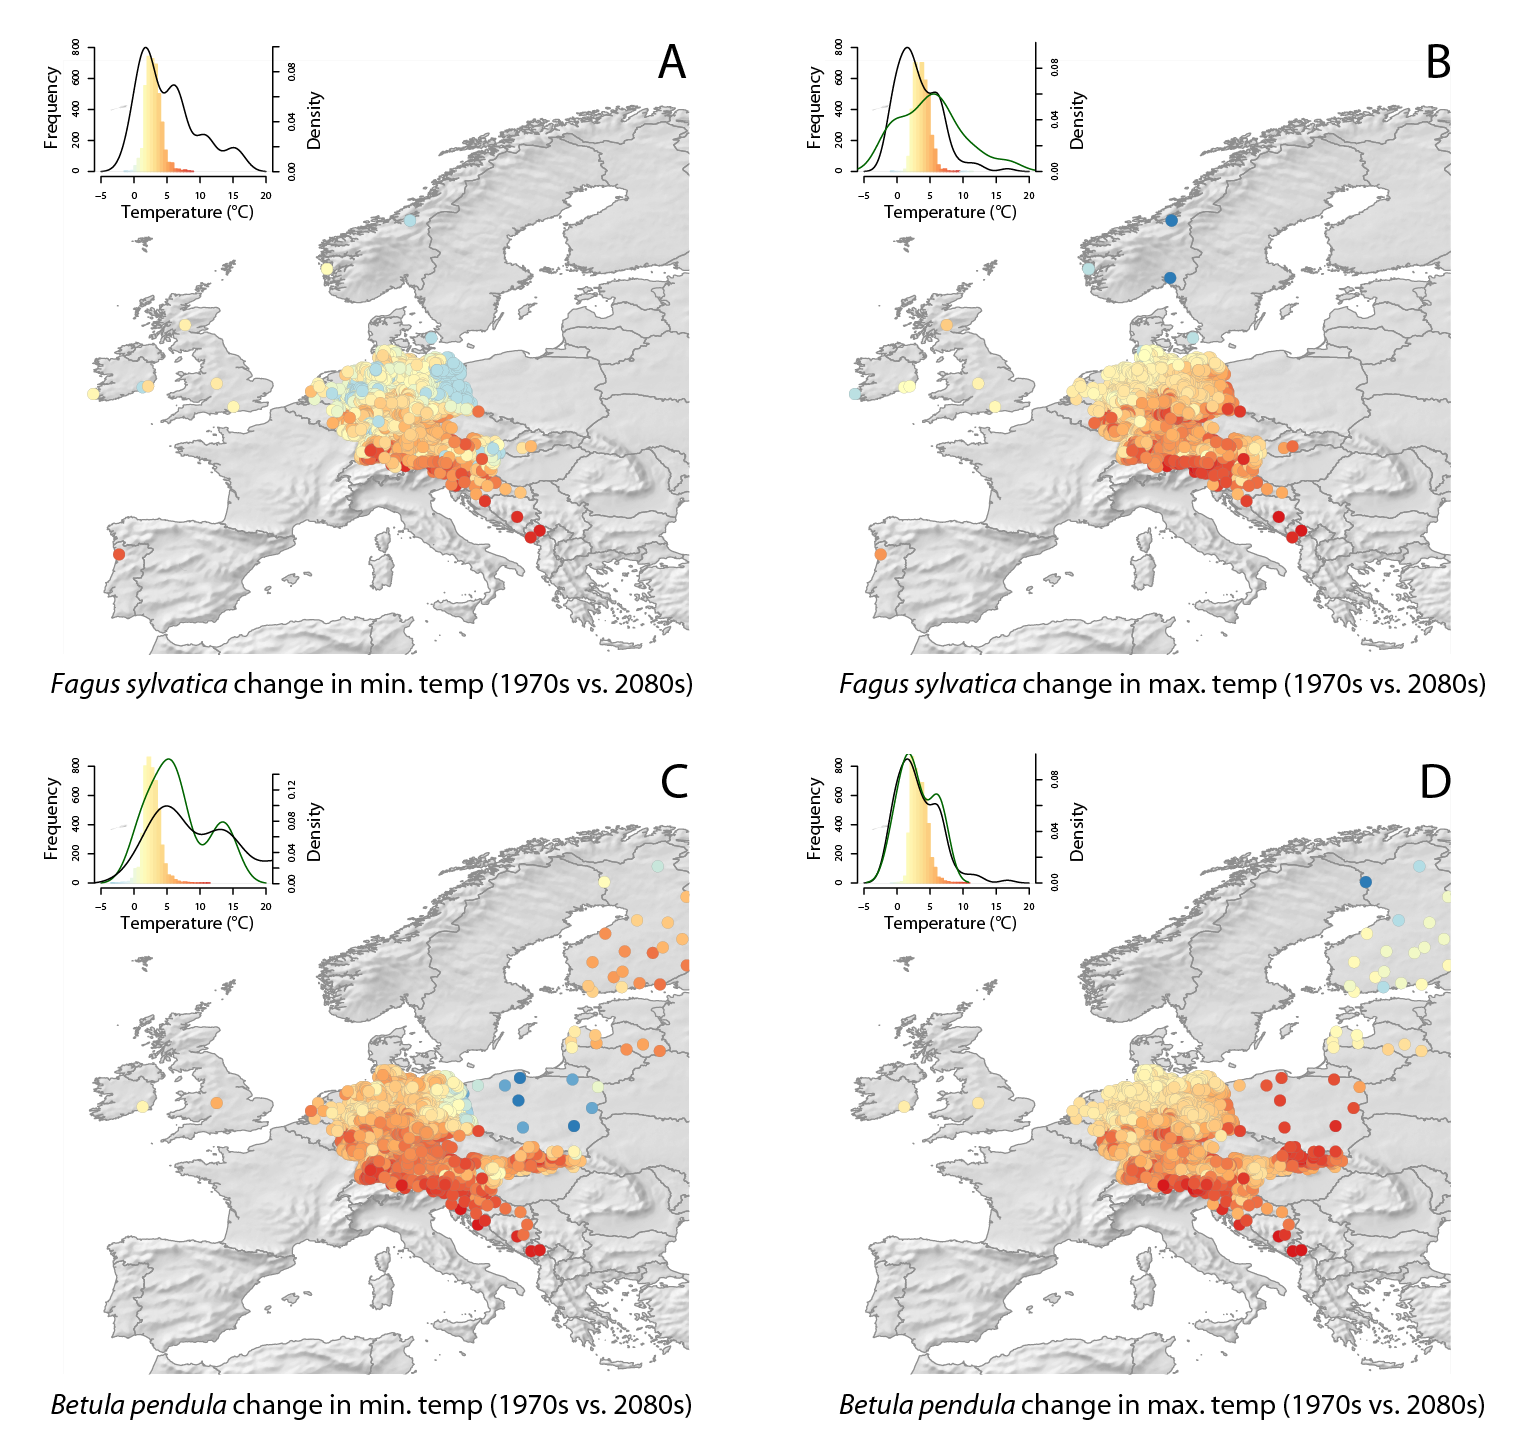
\includegraphics[width=1\textwidth]{figures/Fig1_noblues_densities.png}
\caption{Predicted changes in temperatures relevant to chilling (A, C) and forcing (B, D) compared to a 1970s baseline shown for two species: \emph{Fagus sylvatica} (A-B) and \emph{Betula pendula}. Points represent a PEP725 site with XX data. Inlay plots in the upper left-hand corner of each plot show a histogram of the predicted changes in temperature overlaid with densities of the chilling (A, C) and forcing (B, D) treatments (green lines show the treatments for that exact species, while black lines show across all species; note that for \emph{Fagus sylvatica} there are no chilling treatments of differing temperatures.}
  \label{fig:pep}
\end{figure}
\clearpage


\begin{figure}[t!]
\centering
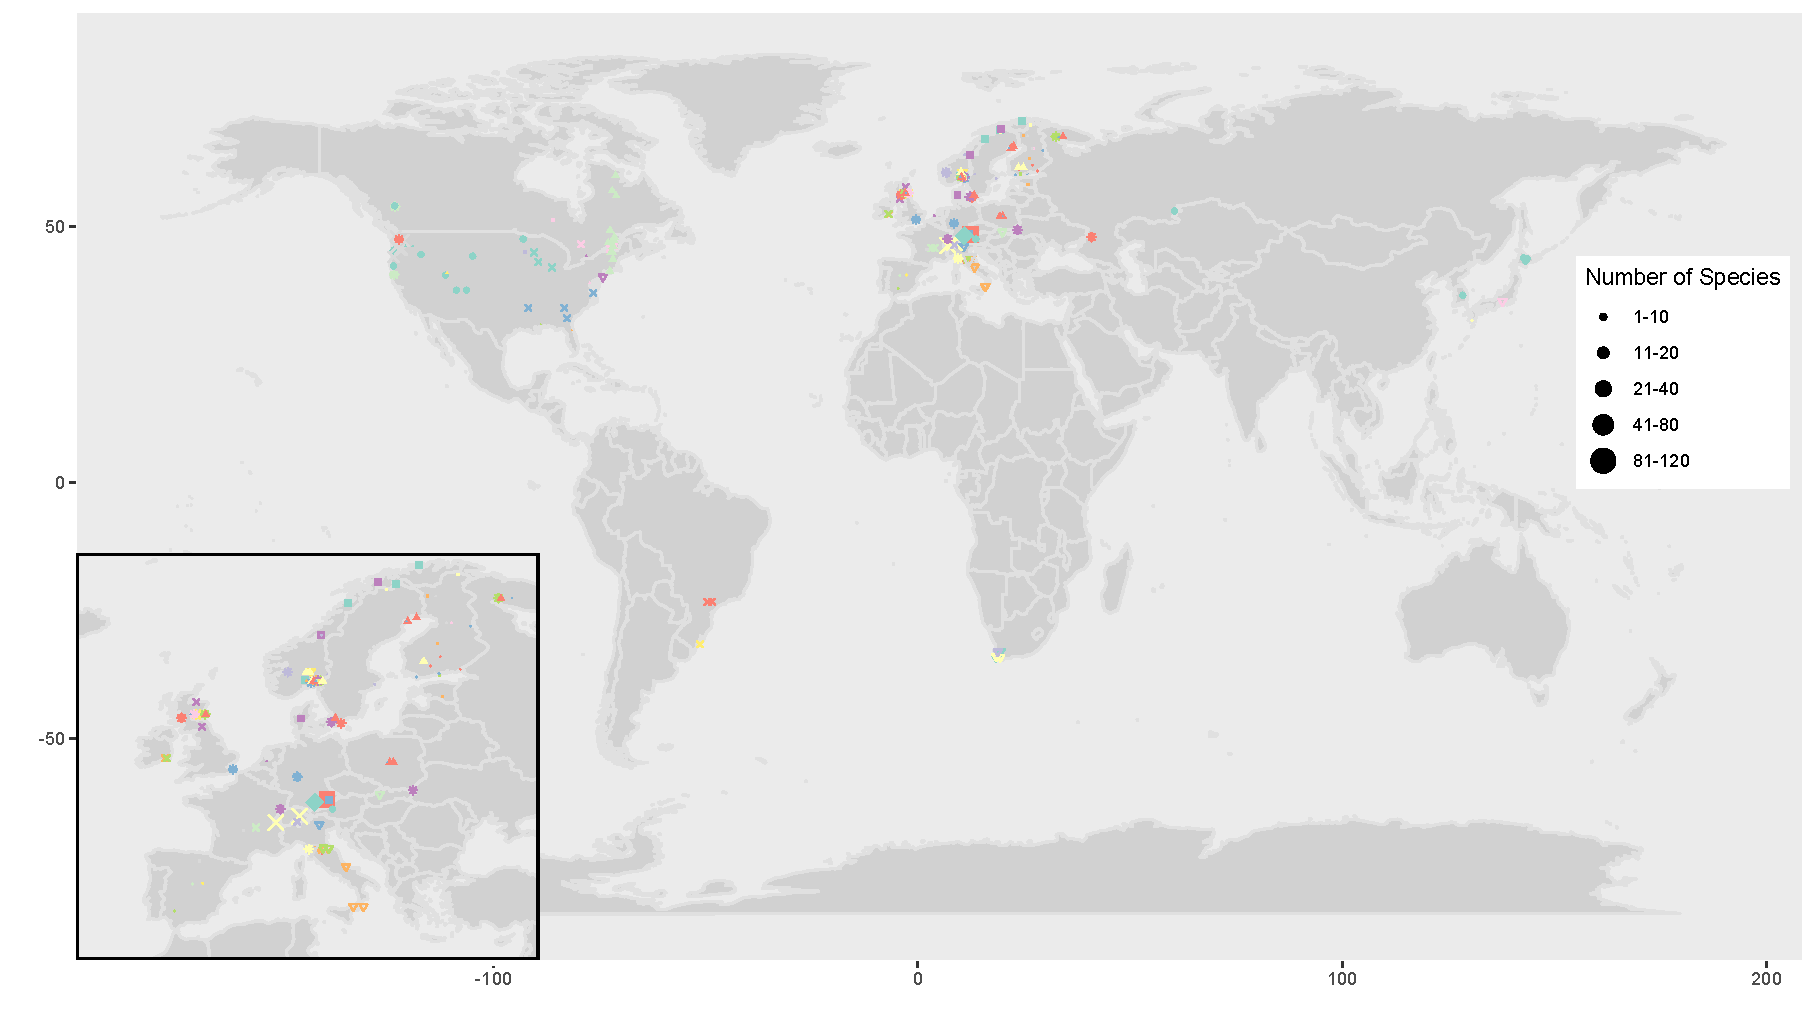
\includegraphics[width=1\textwidth]{..//..//analyses/limitingcues/figures/maps/map_studyspp.pdf}
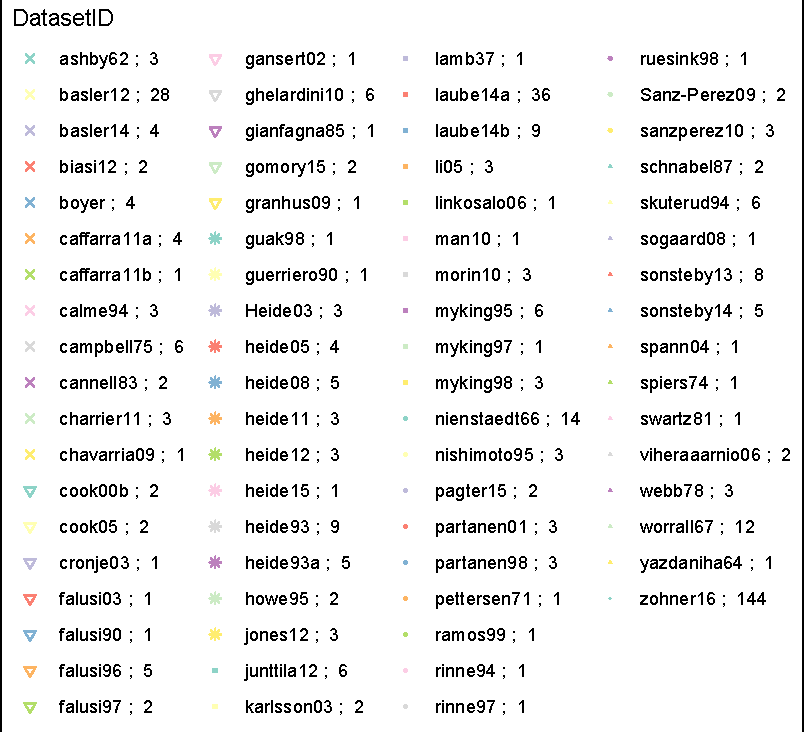
\includegraphics[width=0.5\textwidth]{..//..//analyses/limitingcues/figures/maps/map_studyspp_legend.pdf}

\caption{Overview of the data across space.}
  \label{fig:datamap}
\end{figure}
\clearpage

\begin{figure}[t!]
\centering
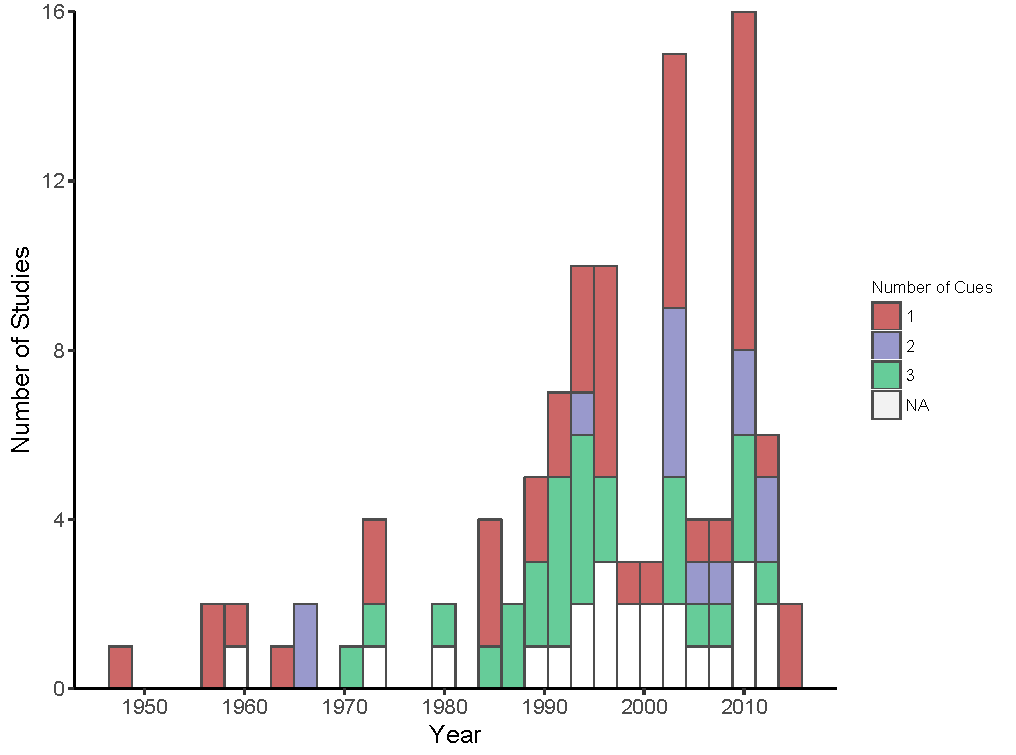
\includegraphics[width=1\textwidth]{..//..//analyses/limitingcues/figures/studyyearcues.pdf}
\caption{Cues manipulated over time.}
  \label{fig:ts}
\end{figure}
\clearpage

\begin{figure}[t!]
\centering
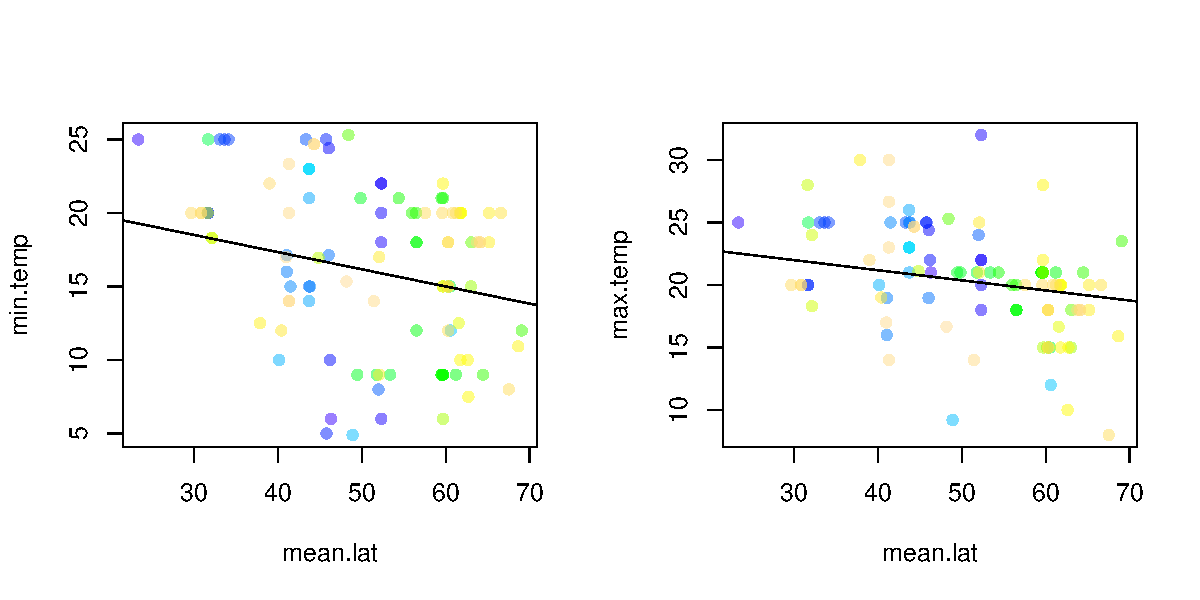
\includegraphics[width=1\textwidth]{..//..//analyses/limitingcues/figures/tempxlatminmaxcorr.pdf}
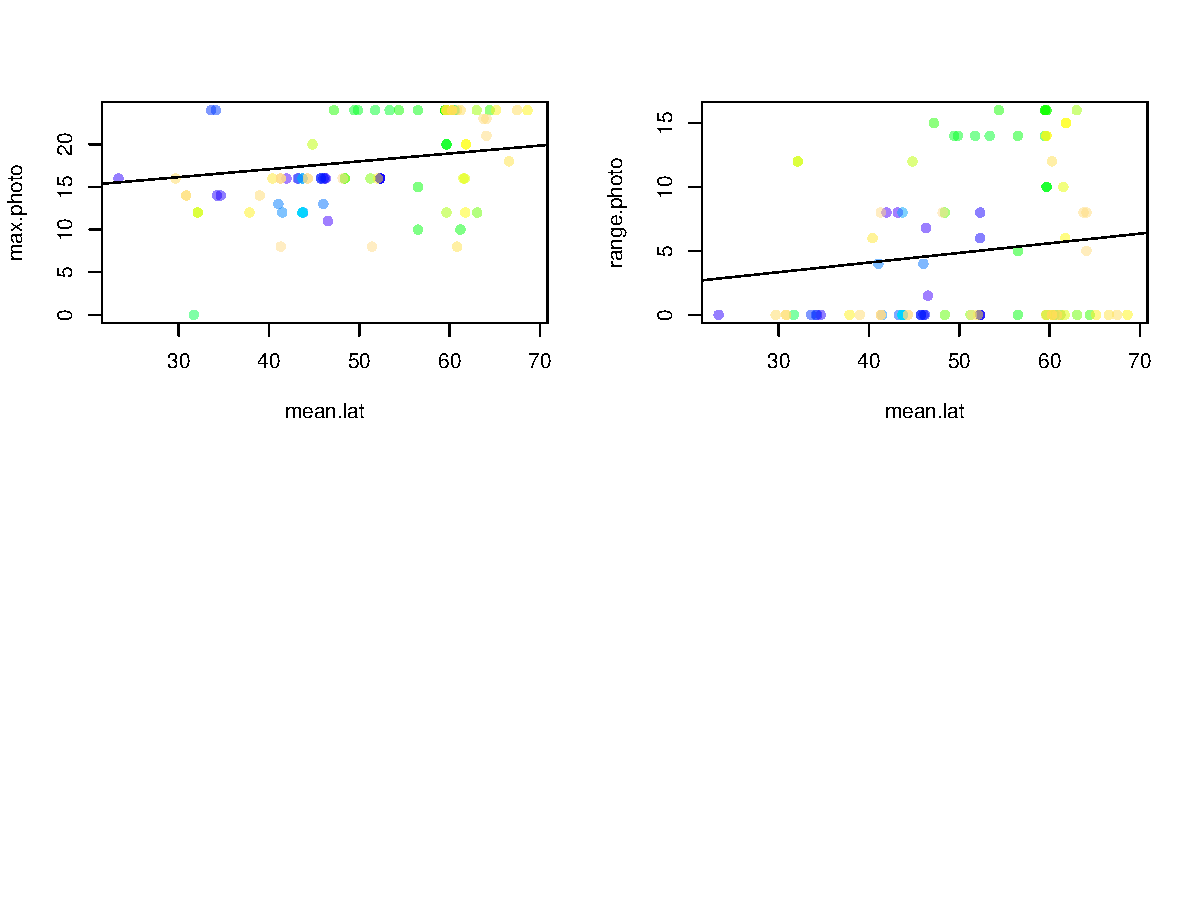
\includegraphics[width=1\textwidth]{..//..//analyses/limitingcues/figures/photoxlatcorr2plots.pdf}
\caption{One correlation with latitude plot? Or more?}
  \label{fig:lat}
\end{figure}
\clearpage

\begin{figure}[t!]
\centering
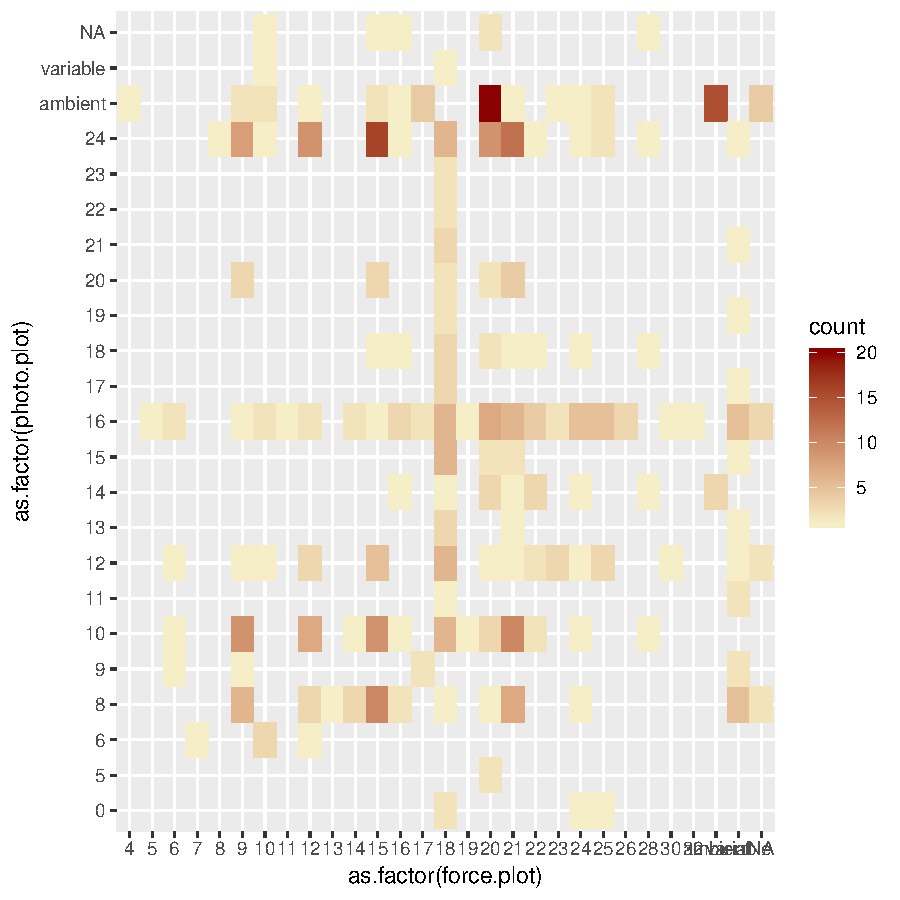
\includegraphics[width=0.3\textwidth]{..//..//analyses/limitingcues/figures/heatmapforcexphoto.pdf}
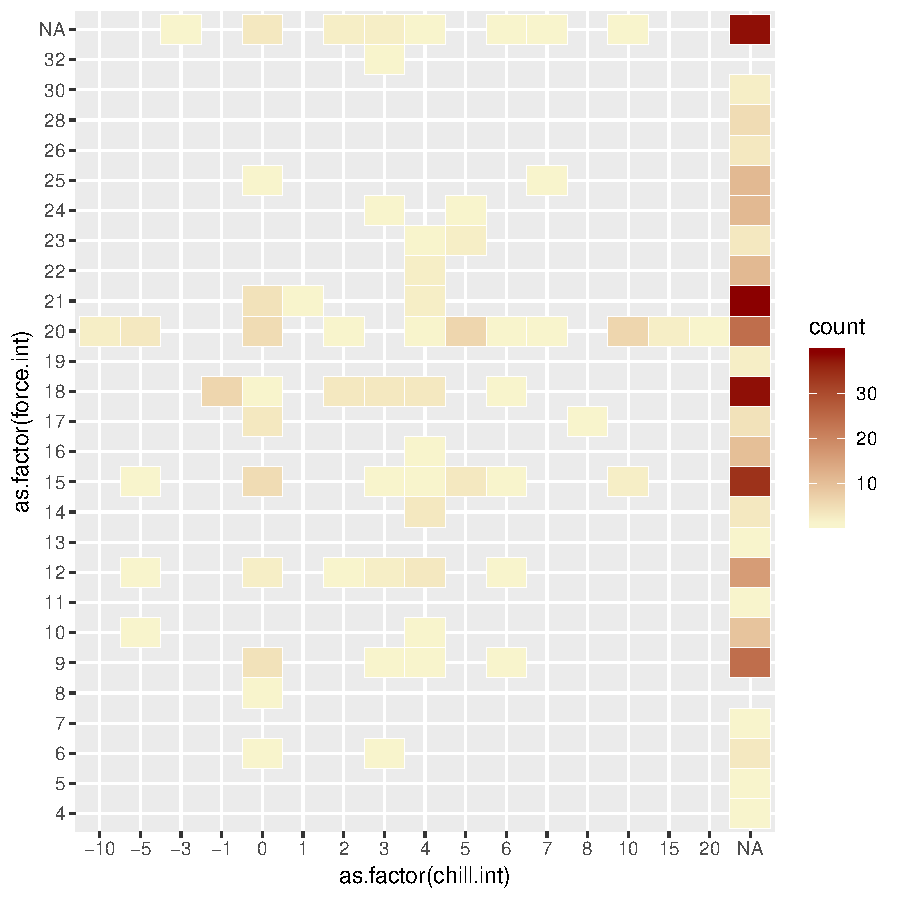
\includegraphics[width=0.3\textwidth]{..//..//analyses/limitingcues/figures/heatmapchillxforce.pdf}
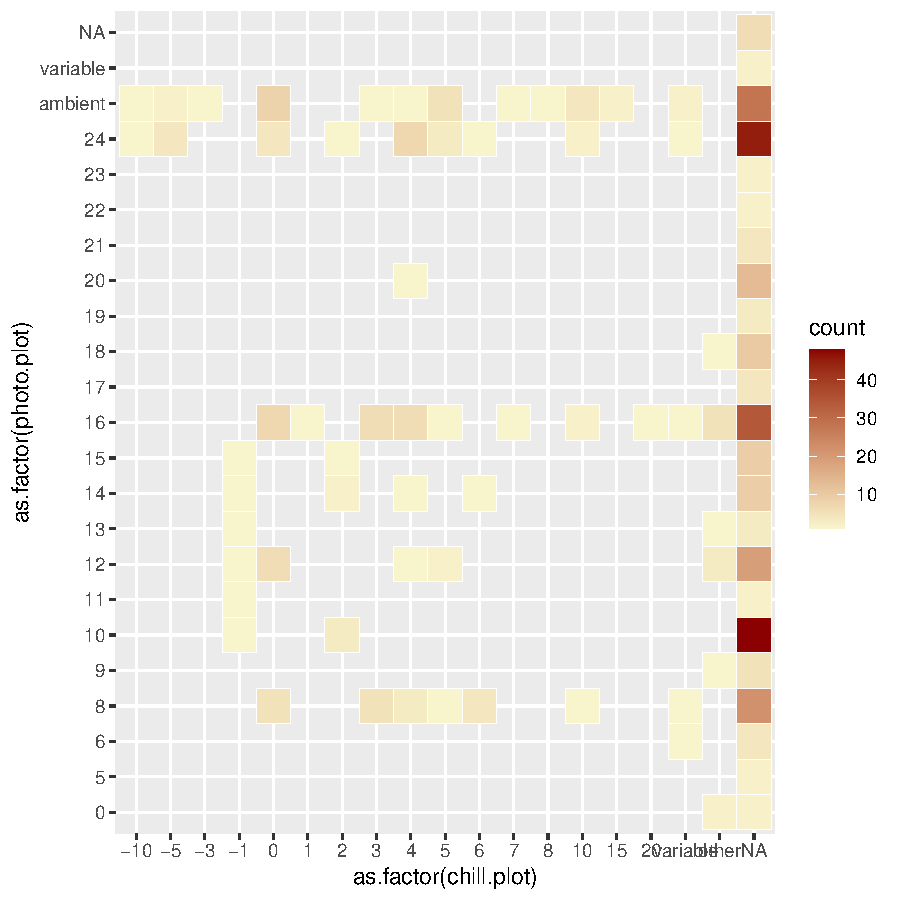
\includegraphics[width=0.3\textwidth]{..//..//analyses/limitingcues/figures/heatmapchillxphoto.pdf}
\caption{Heat maps.}
  \label{fig:heatmaps}
\end{figure}
\clearpage



\end{document}
%%%%%%%%%%%%%%%%%%%%%%%%%%%%%%%%%%%%%%%%%%%%%%%%%%%%%%%%%%%%%%%%%%%%%%%%


%=======================================================================
% to-do listing
%=======================================================================

\listoftodos

%=======================================================================
\section*{Other loose ends}
%=======================================================================


\section*{Extended notes on local adaptation vs. plasticity}

Relevant lit to when you do and don't see local adaptation:
\begin{enumerate}
\item \citet{kelly2003}: the impact of yearly variation in temperatures in genotype selection % "we have found within a naturally occurring stand of the tree species Betula pendula (birch) a regular occurrence of genetic segregation correlating with normal year-to-year variation in mean annual temperature"
\item High variation in spring climatic conditions makes temporal variation in many ways as high as spatial and thus may slow local adaptation \citep[see also ][]{legave2013} (also note that geneflow across space will shape phenological cues)
\end{enumerate}
\item A species' range limit and its phenology are intertwined: a species' current range defines the range of cues it may see, but phenology also shapes those limits \citep{morin2007,Morin:2008vp}.
%  New term: Cue range limits. What do you think? As in the limits of cues as seen over a species' range, what do you think?
%% IMC - I love this idea of Cue range limits, and I guess it is somewhat linked to what X. Morin and I. Chuine have been working on, given that their process-based models would predict species range shifts based on the effects of cues on phenology

\section*{Old notes on thermal tolerances.}

Thus you may consider thermal tolerances/limits (and where is the species optimum?) when designing growth chamber studies  ...These tests could be especially useful for understanding range limits: look at treatments beyond the variation seen within a species' range and see if there is abrupt change or you see continuous change, if no abrupt change then it may suggest that something else must limit range (e.g., biotic cues, minima temperature after which species) 
(IMC): Above is true, but perhaps it is far afield. If we decide to leave it in, I would consider emphasizing the fact that while thermal physiology is receiving increased attention to delineate species ranges, for trees that sort of information may not be particularly insightful given the following reasons: (a) there's still little data on CTmax and CTmin for a majority of tree species, (b) there are not huge differences in those thermal tolerances among tree species, and (c) a given tree species may tolerate very high or low temperatures before it dies, but if its phenology advances (or delays) too much, it may cease to reproduce. 

